% Drawing 144/04-1 -- folder 144, batch 04, archive page 62 (PDF page 63).
% Transcription: Une sphère, coupée par l'équateur ; sur l'équateur, les points $0$, $1$, $\infty$ et les arcs $K_0$, $K_1$, $K_\infty$ (ce dernier, de $0$ à $1$, renforcé) ; l'hémisphère supérieur marqué $\Gamma_+$, l'inférieur $\Gamma_-$, avec une flèche d'orientation.
% Kind: sphere cut by the equator: arcs K_0, K_1, K_infty. Method 2 (schematic redraw from the facsimile). Status: ok.
% Notes: The arc K_infty from 0 to 1 is reinforced (thick); infinity at the back; Gamma_+ above, Gamma_- below; an orientation arrow on the lower left.
% Coordinates: 1 unit = 1 mm = 1/100 of the crop width (bbox in page fractions: [0.1, 0.17, 0.32, 0.31]).
% Redrawn by Claude (claude-opus-5-5), issue #73, 2026-11-07; not checked by a human; not compiled (no TeX in the session).
% Rights: reproduces part of the work -- behind RENDER_TRANSCRIPTS, never published by itself.
\documentclass[tikz,border=3pt]{standalone}
\usepackage{amsmath,amssymb}
\usetikzlibrary{patterns,arrows.meta}
\tikzset{pencil/.style={black!45}, struck/.style={black!35}, mark/.style={circle,draw,inner sep=1.3pt}, pt/.style={circle,fill,inner sep=0.9pt}, opt/.style={circle,draw,fill=white,inner sep=1.1pt}}
\begin{document}
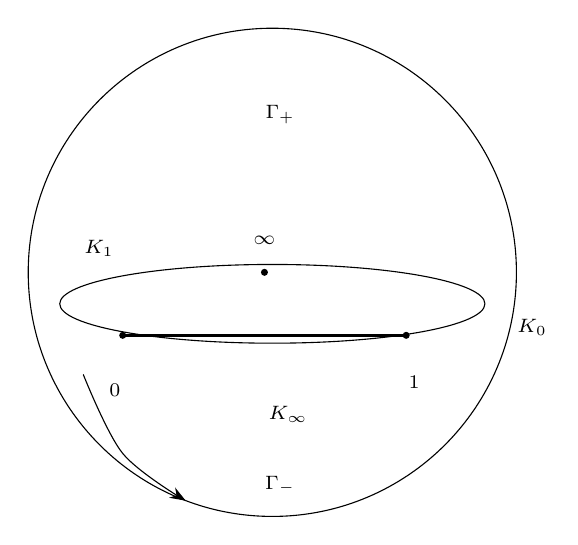
\begin{tikzpicture}[x=1mm,y=1mm,line cap=round,line join=round,font=\scriptsize]
\draw (43,-47) circle[radius=31];
\draw (43,-51) ellipse[x radius=27, y radius=5];
\draw[very thick] (24,-55) -- (60,-55);
\node[pt] at (24,-55) {};
\node[pt] at (60,-55) {};
\node[pt] at (42,-47) {};
\node[inner sep=1pt] at (23,-62) {\scriptsize $0$};
\node[inner sep=1pt] at (61,-61) {\scriptsize $1$};
\node[inner sep=1pt] at (42,-43) {\scriptsize $\infty$};
\node[inner sep=1pt] at (44,-27) {\scriptsize $\Gamma_+$};
\node[inner sep=1pt] at (44,-74) {\scriptsize $\Gamma_-$};
\node[inner sep=1pt] at (21,-44) {\scriptsize $K_1$};
\node[inner sep=1pt] at (76,-54) {\scriptsize $K_0$};
\node[inner sep=1pt] at (45,-65) {\scriptsize $K_\infty$};
\draw[-{Stealth[length=2mm]}] plot[smooth, tension=0.55] coordinates {(19,-60) (24,-70) (32,-76)};
\end{tikzpicture}
\end{document}
